\section{System Design Specification}

\begin{figure}[!h]
    \centering
    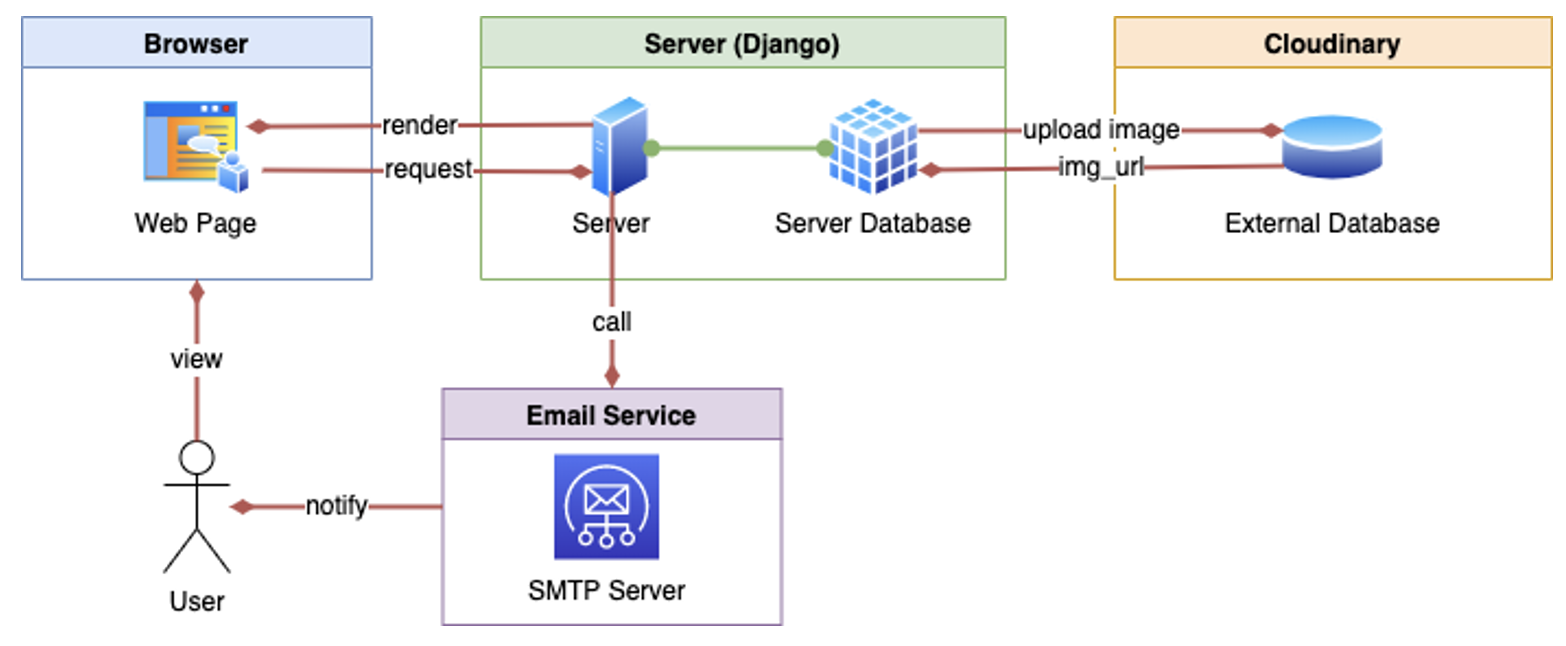
\includegraphics[scale=0.6]{figures/arch.png}
    \caption{Architecture Overview of DAP}
    \label{fig: arch}
\end{figure}

The system is designed with specific security consideration which will be introduced in this section. Overall, DAP is a client-server system and there is no direct communication between clients. The server will get involved in all activities. Therefore, we do not need to consider about P2P protocol and security. As a client-server system, DAP has a back-end and a front-end. Front-end code provides interaction entries and get/post data to the server, whereas back-end stores information of artwork and handles encryption/decryption. The architecture is depicted in Fig. \ref{fig: arch}. We implement DAP based on Python Django Web framework\footnote{https://www.djangoproject.com/}.

\subsection{Security assumptions}\label{sec:assumption}

Similar as any system, our discussion on security of DAP is base on several assumptions:
\begin{enumerate}
\item The front-end of the system could be accessed by the public.
\item The private key and user data in server cannot be hacked
\item Third party services like cloudinary is trustworthy
\item The communication between the platform and the user could be insecure.
% \item todo, if any
\end{enumerate}

\subsection{Authentication and authorization}
\label{sec: aa}

As a online platform, it is important to have an authentication mechanism. We use the authentication system provided by Django. Django authentication system handles both authentication and authorization. In the context of Django, authentication verifies that a user is who they claim they are, whereas authorization determines what permissions does an authenticated person have.

A model in Django is the single, definitive source of information about data. Each model maps to a single database table. To be more specific,

\begin{itemize}
    \item Each model is a Python class that subclasses django.db.models.Model.
    \item Each attribute of the model represents a database field.
\end{itemize}

User models are the core of the authentication system. Clients and administrators are the two types of users that interact with DAP. For administrators, they are allowed to access the admin page and view/modifiy our database. DAP does not store raw (plain text) passwords on the user model, but only a hash. Therefore direct manipulation of the user's password properties is not allowed, even for administrators. By default, Django uses the PBKDF2 \cite{kaliski2000pkcs} algorithm with a SHA256 hash to store passwords, which is a password stretching mechanism from RSA Laboratories’ Public-Key Cryptography Standards series recommended by NIST. This should be sufficient for DAP: it’s quite secure, requiring massive amounts of computing time to break. Keys of PBKDF2 are encrypted based on RSA and stored in Django admin database. 

\subsection{Communication}

We use HTTPS for communication. The main underlying protocol under HTTPS is TLS, which implements an mechanism similar to strong password protocol to ensure security. The difference is that, TLS requires the server to have an certification, which will help prove the identity of server. As a consequence, only server needs to have a private key in TLS. Without the use of HTTPS/SSL, malicious web users could sniff authentication credentials or any other information transmitted between client and server, and in some cases, active web attackers could change data sent in either direction.

Besides HTTPS, since DAP use email to deliver messages, we also need to concern the security of email as a data transfer method.  

By default, SMTP does not include encryption of data. However, the email data should be protected in our application. Pretty good privacy (PGP)\cite{network2007openpgp} is one of the possible solution to add security level. Basically, PGP use a combination of cryptographic functions to sign and encrypt the text. We use PGP to protect the email content, so that the content could only be decrypted by the receiver. Example see Fig \ref{fig:pgp}.

\begin{figure}
    \centering
    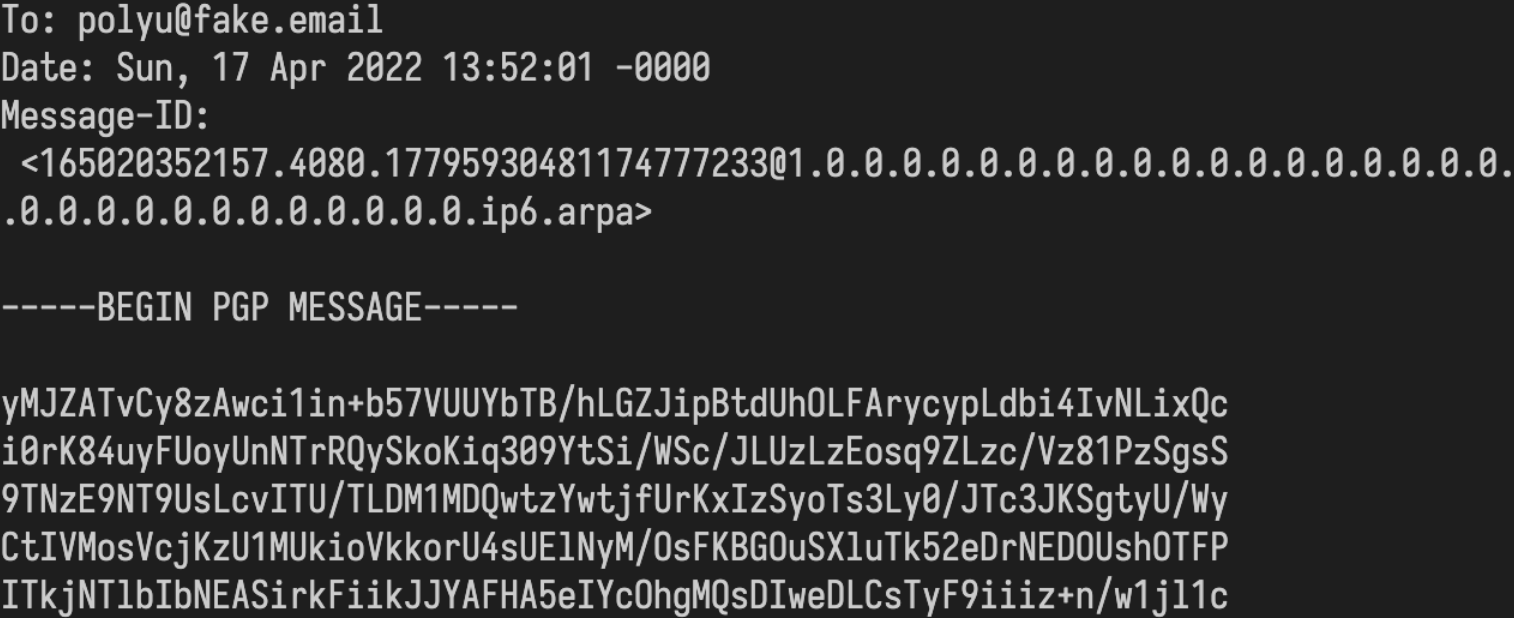
\includegraphics[scale=0.6]{sections/pgp-ex.png}
    \caption{An example of PGP encrypted email (partly)}
    \label{fig:pgp}
\end{figure}

Apart from PGP still provide some encryption level to the email. When we are communicating with the SMTP server, we use TLS (Transport Layer Security) provided by Django\footnote{ https://docs.djangoproject.com/en/4.0/ref/settings/#email-use-tls} to encrypt the data.
\subsection{User data}

% As mentioned in \ref{sec: aa}, DAP stores users' data in the user models. Additionally, there are other models that contain user data, such as transaction models. For these users' data, DAP applies ... .

When user uploads a artwork, we calculate and store locally the hash of the file. Such hash is used to check the integrity of the file when we further fetch it from cloudinary. This design follows our discussion about integrity in section \ref{sec:integrity}.

For the content of artwork, as mentioned in Sec \ref{sec:confiden}, does not necessarily to be encrypted. We store artworks in cloudinary, which additionally provides some safety mechanism (they do not release the detail).  
\subsection{Digital artwork}

As a digital artwork platform, digital artwork themselves are stored in a third-party platform called cloudinary\footnote{https://cloudinary.com/}, who has their own mechanisms to ensure the safe storage. After a user post his/her digital artwork \textit{DA1}, DAP will call cloudinary api to transfer \textit{DA1} securely (via HTTPS). Then, cloudinary will store \textit{DA1} together with a digital signature in their database. Finally, cloudinary will reply a secure link (also HTTPS) of \textit{DA1} to DAP and DAP will store this link as part of user data. Users with successful authentication can view \textit{DA1} via this link. \par

Due to business and security concerns, cloudinary does not disclose too much specific security mechanisms to developers, but using the services they provide is still one of our safest choices, which also matches the assumption at Sec \ref{sec:assumption}.

The ownership information (OI) is important to generate digital signature (DS) on digital artwork. OI is created/modified when the owner post their digital or a transaction is done, and DS will be changed in cloudinary storage simultaneously.  Along with other user data stored in user models, OI is also protected in our database.

\subsection{Transaction}
Transaction in a higher level of abstraction means the change of ownership. It does not necessarily invloves any format of currency. In our DAP, we currently do not include real payment APIs for some commercial issues. In our current setting, users has rights to transfer the ownership of an artwork to another user. Users could also request transfer of artwork, and if the owner agree, the transaction could be done.
